\documentclass[10pt,journal]{IEEEtran}
\usepackage{microtype}
\usepackage{amsmath,amssymb,mathtools}
\usepackage{booktabs,multirow,array}
\usepackage{graphicx}
\usepackage{cite}
\usepackage{xcolor}
\usepackage{url}
\renewcommand{\baselinestretch}{0.88}
\emergencystretch=1em
\setlength{\textfloatsep}{5pt plus 1pt minus 1pt}
\setlength{\floatsep}{4pt plus 1pt minus 1pt}
\setlength{\intextsep}{5pt plus 1pt minus 1pt}
\setlength{\abovedisplayskip}{3pt plus 1pt minus 1pt}
\setlength{\belowdisplayskip}{3pt plus 1pt minus 1pt}
\renewcommand{\arraystretch}{0.94}
\newcommand{\RiskSafe}{risk-constrained verifier}
\newcommand{\TailRisk}{tail-risk counterfactual}
\newcommand{\PaymentSafe}{payment-certified verifier}
\newcommand{\dt}{\Delta t}

\title{Security-Aware Workload-State Counterfactual Verification and\\
Nodal Net-Value Settlement for Spatially Coupled AI Data Centers}
\author{Anonymous Authors}

\begin{document}
\maketitle

\begin{abstract}
Artificial-intelligence (AI) data centers can provide demand response (DR),
but a meter-only baseline cannot distinguish a realizable workload shift from
strategic deferral, rebound, or a transmission-feasible response. We present a
security-aware workload-state verifier and nodal settlement that link a
committed job ledger, feasible service trajectories, and contingency-constrained
network value. A sparse multi-period linear program enforces release,
conservation, deadlines, capacity, migration, and cross-midnight completion.
A validation-only convex quadratic program with a linear false-credit/CVaR
epigraph and a two-sided event band gives an auditable risk contract; an
event-gate mode never credits unsubmitted future work. Signed dispatch-value
differences under finite non-islanding single-contingency (N--1) constraints
determine payments, with exact coalition accounting for allocation. On
5,188,507 BurstGPT requests and 71,128 positive-energy MIT Supercloud jobs,
the risk-constrained verifier reduces unsupported credit from 1.849211 to
1.826322 MWh/day (1.24\%) relative to the selected single feasible cap, while
its nRMSE changes from 0.345209 to 0.345019. Relative to the feasible-quantile
comparator, unsupported credit falls by 37.40\% (2.917471 to 1.826322
MWh/day); exact three-day block tests are reported without claiming uniform
accuracy improvement. Exact N--1 settlement reduces trace-anchored error from
\$165.288 to \$1.018/day across 37 RTS-24 outages, while end-to-end errors are
\$192.978, \$159.514, and \$159.483/day for base-case exact, N--1 linear, and
N--1 exact settlement. Independent replay covers every locked 15-minute slot and
job-level residuals are below $10^{-17}$ MWh. Held-out conversion endpoints,
four public AC networks, spatial permutations, and a workload-hull payment
interval test the declared uncertainty boundary. The non-co-located public
traces define a reproducible benchmark, not a utility field event.
\end{abstract}

\noindent\textbf{Index Terms---}AI data centers, counterfactual verification,
demand response, security-constrained dispatch, nodal settlement.

\section{Introduction}

The growth of large-model training and inference is converting data centers
from nearly static industrial loads into large, software-defined grid
resources. Interactive inference is latency constrained, elastic inference can
be delayed briefly, and batch GPU work can be deferred for hours or migrated
between regions. These capabilities enable demand response (DR), but they also
invalidate the usual interpretation of a meter decrease. A reduction at one
facility can be followed by delayed consumption or simultaneous rebound at
another node. Paying the positive local decrease can therefore reward a
redistribution that creates little or negative network value.

Conventional DR measurement and verification estimates the unobserved
no-event demand from historical meter data. Arithmetic historical baselines
remain common in market practice, despite known bias and manipulation
incentives \cite{wang2022baseline,caiso2017baseline}. Regression-based facility models quantify
baseline uncertainty but do not encode a computing workload ledger
\cite{wang2022baseline}. More broadly, DR
research establishes the economic role of responsive load, yet a meter-only
estimator cannot determine whether queued jobs could actually have produced
its predicted trajectory.

Data-center scheduling studies provide the missing physical state. Temporal
deferral, dynamic capacity, and geographical load balancing can reduce energy
cost and peak demand \cite{liu2013dcdr}. Geographical assignment provides the
complementary spatial control mechanism \cite{adnan2012geographical}. Recent
work assesses data-driven flexibility and aggregator coordination
\cite{cao2022flexibility,zhang2024aggregator}, while multi-level dispatch
refines delay-sensitive electrical response.
Hierarchical optimal-consumption models further connect facility efficiency
with response quality \cite{zhou2025loadmodel}.
Virtual-link market clearing and space--time remuneration establish how
geographical and temporal transfers can enter electricity markets
\cite{zhang2020virtuallinks,zhang2022remunerating}. Receding-horizon operation
and uncertainty-aware frequency-regulation coordination further establish the
need to retain future arrivals and multi-site state
\cite{zhang2023receding}. However, these methods optimize
an operator-controlled schedule rather than verify an independently submitted
DR counterfactual against an auditable workload ledger. This separation between
computing feasibility and market verification motivates the auditable ledger
used here.

The second gap is electrical. Geographic workload control is commonly valued
with energy prices or gross megawatts. Such accounting ignores the fact that
nodal marginal value changes when congestion or a contingency constraint
binds. Direct-current (DC) power flow and linear distribution factors provide transparent
network sensitivities \cite{stott2009dc,zimmerman2011matpower}; N--1 dispatch
can impose every credible post-contingency line limit through line-outage
distribution factors (LODFs) \cite{tejada2018lodf}. No existing data-center DR
verification framework jointly certifies workload feasibility, preserves
signed spatial response, and settles the resulting security-aware network
value. Public workload and facility telemetry can support an observational
replay of that ledger, but it does not constitute a causal utility event; a
rigorous study must therefore separate measured-execution replay, counterfactual
construction, and network-value verification rather than present them as one
field intervention.

This paper makes three power-system contributions. 1) We formulate a
provenance-bound workload-state demand model in which release, deadline,
conservation, cross-midnight completion, capacity, and migration constraints
are enforced simultaneously. The resulting job-level witness links each
joined job to its immutable scheduler/DCGM record and preserves measured
execution energy. 2) We construct a validation-only, continuous-arrival
counterfactual verifier with a pointwise credit envelope. The output is an
attainable spatial--temporal load trajectory rather than an unconstrained
meter-only prediction, and its statistical performance is evaluated under an
explicit false-credit/under-credit tradeoff. 3) We develop signed
space--time nodal remuneration and a bilateral net-value contract under
preventive N--1 dispatch, and map the feasible workload set into a payment
uncertainty interval over held-out workload-to-power conversion. The novelty is
the coupling invariant that carries one committed workload state into physical
verification, network valuation, and a set-valued settlement rule; the
individual LP, dispatch, and allocation primitives are standard and are not
claimed as new in isolation. The certificate is conditional on trusted
scheduler and telemetry provenance: a cryptographic digest verifies record integrity after
commitment but does not authenticate semantically false fields.

The remainder of the paper is organized as follows. Section~\ref{sec:model}
defines the spatial workload and network settlement problem. Section~\ref{sec:method}
presents the verifier, security-aware value rule, and allocation mechanism.
Section~\ref{sec:design} specifies the data, baselines, and locked protocol.
Section~\ref{sec:results} reports the core counterfactual, execution-replay,
job-level, security, payment, continuous-horizon, and provenance experiments.
Section~\ref{sec:conclusion} concludes with the deployment boundary and future
validation requirements.

\section{System Model and Problem Formulation}\label{sec:model}

\subsection{Spatial workload state}

Let $\mathcal S$, $\mathcal K$, $\mathcal D$, and $\mathcal T$ denote source
regions, workload classes, destination data centers, and 15-minute intervals.
The measured ledger supplies arrival energy $a_{skt}$ for source $s$, class
$k$, and release interval $t$. The decision $x_{skd\tau}\geq0$ is the energy
served at destination $d$ in interval $\tau$. Its cumulative state is
\begin{equation}
 y_{skt}=\sum_{\tau=0}^{t}\sum_{d\in\mathcal D}x_{skd\tau}.
 \label{eq:cumulative}
\end{equation}
With cumulative arrivals $A_{skt}=\sum_{\tau=0}^{t}a_{sk\tau}$ and deadline
$D_k$, release and deadline feasibility are
\begin{align}
 y_{skt}&\leq A_{skt}, \label{eq:release}\\
 y_{skt}&\geq A_{sk,t-D_k},\quad t\geq D_k. \label{eq:deadline}
\end{align}
The state recursion equals service, terminal service equals total arrivals, and
$\sum_{s,k}x_{skdt}\leq\bar P_d\dt$. Facility demand is
\begin{equation}
 p_{dt}=P_d^{\rm fix}+\dt^{-1}\sum_{s,k}x_{skdt}.
 \label{eq:power}
\end{equation}
For rolling window end $T^+$ and final event-day release $T^0$, the terminal
state is not forced to consume unexpired future work. Instead,
\begin{equation}
y_{skT^+}=A_{sk,\max\{T^0,T^+-D_k\}},
\label{eq:rollingterminal}
\end{equation}
which completes every job due inside the window and every event-day arrival,
while retaining later real arrivals in the release constraints. The window
starts $D_{\max}+96$ intervals before the event day and ends $D_{\max}$
intervals after it; omitted earlier work must therefore expire before the
evaluated day.
Equations (\ref{eq:release}) and (\ref{eq:deadline}) prevent early execution
and late completion, while (\ref{eq:power}) maps the feasible service state to
the facility meter.
This model follows workload deferral and geographical assignment foundations
\cite{liu2013dcdr,adnan2012geographical}; its rolling implementation follows
the state-retention principle in \cite{zhang2023receding}. Waiting and migration costs are
$w_k(\tau-t)x_{skd\tau}$ and $m_{sd}x_{skd\tau}$, respectively. Because
arrivals are fixed, replacing waiting duration by service time adds only a
constant.

For provenance, each retained job is represented by the canonical tuple and
its digest in
\begin{equation}
\begin{aligned}
 \ell_j={}&(\mathrm{id}_j,t_j^{\rm submit},t_j^{\rm start},t_j^{\rm end},
 E_j,n_j^{\rm tel},q_j,\kappa_j,\sigma_j),\\
 \mathcal L={}&\operatorname{sort}\{\ell_j:j\in\mathcal J\},\\
 h_{\mathcal L}={}&\operatorname{SHA256}\!\left(\operatorname{serialize}(\mathcal L)\right).
\end{aligned}
\label{eq:ledgerdigest}
\end{equation}
where $E_j$ is the positive aggregated Data Center GPU Manager (DCGM)
energy and $n_j^{\rm tel}$ is its raw telemetry-record count. The digest uses
the Secure Hash Standard \cite{nist2015fips1804}; the canonical row order,
one-to-one join, release--execution order, and raw-to-join energy equality are
checked independently of the scheduling linear program (LP). Consequently, the flow witness
certifies the exact committed ledger and measured profile, while the digest
does not make an unverified claim about jobs that might have been submitted
before the commitment. Experiment~16 reports this provenance certificate and
reconciles the measured regional capacity envelope with the 118-MW nameplate
that was committed before the validation/test split; the envelope is not used
to select that nameplate.

The trust boundary is explicit. The verifier assumes that the scheduler and
DCGM services are the authoritative sources for the fields used in
\(\ell_j\), and that the digest is committed before the event decision. Under
this assumption, a changed record is detectable and a joined record cannot be
silently replaced after commitment. The digest does not, however, establish
that a semantically false deadline, region label, service class, or energy
value was truthful when it was signed. Authenticity of those fields requires
an upstream scheduler attestation, meter signature, or trusted execution
interface; it is outside the optimization certificate proved here.

\subsection{Counterfactual, response, and false credit}

For event set $\mathcal E\subset\mathcal T$, $p^0_{dt}$ denotes the no-event
counterfactual and $p^1_{dt}$ denotes the event trajectory generated by the
declared workload optimization. The mechanism-isolation experiments use
$p^{1,\mathrm{sim}}$ for this optimized response, whereas Experiment~13
uses $p^{1,\mathrm{meas}}$ for the independently measured MIT/DCGM execution
trace. We reserve $p^{\rm obs}$ for measured execution used only as scoring
truth; it is never supplied to an estimator or used to claim a causal utility
event. For either response trace, $r_{dt}=p^0_{dt}-p^1_{dt}$ is signed:
gross local response is $[r_{dt}]_+$, while net response retains negative
rebound. For an estimate $\widehat p^0$, unsupported credited energy is
\begin{equation}
 F=\dt\sum_{d,t\in\mathcal E}
 [\widehat p^0_{dt}-\max\{p^{\rm obs}_{dt},p^1_{dt}\}]_+ .
 \label{eq:falsecredit}
\end{equation}
The audit computes (\ref{eq:falsecredit}) separately for every locked day so
that a favorable aggregate error cannot hide unsupported positive credit.
We also report normalized root-mean-square error (nRMSE), bias, precision,
recall, $F_1$, under-credit, payment error, and overpayment.

\subsection{Strategic reference scheduling}

Consider an arithmetic mean of $H=10$ reference days, event probability $q$,
and DR price $\pi^{\rm DR}$. If reference day $j$ adds event-window service
$\delta R_j$, the expected payment change is
\begin{equation}
 \Delta\Pi=\frac{q\pi^{\rm DR}}{H}\sum_{j=1}^{H}\delta R_j
 -\sum_{j=1}^{H}\Delta C_j .
 \label{eq:profit}
\end{equation}
Let $c'_j$ be the right derivative of the minimum operating cost with respect
to an event-window minimum-service constraint on day $j$. Linear-program
sensitivity \cite{boyd2004convex} gives the following exact local condition:
\begin{equation}
\begin{aligned}
 \frac{q\pi^{\rm DR}}{H}>\min_j c'_j
 \quad\Longleftrightarrow\quad {}&
 \exists\ \text{a strictly profitable}\\[-2pt]
 &\text{local deviation}.
\end{aligned}
 \label{eq:threshold}
\end{equation}
The historical-baseline premise is documented in
\cite{wang2022baseline}; (\ref{eq:profit})--(\ref{eq:threshold})
are this paper's workload-specific specialization.

\subsection{Network value}

Let $M$ be the data-center-to-bus incidence matrix and
$p_t=p_t^{\rm native}+Mp_t^{\rm dc}$ the nodal demand vector. For
generator-to-bus map $C_g$, generator bounds, power
transfer distribution factor (PTDF) $H$, and line ratings $\bar f$, the
piecewise-linear security-constrained economic dispatch (SCED) value is
\begin{align}
 V(p)=\min_g\;&\sum_i C_i(g_i) \label{eq:sced}\\
 {\rm s.t.}\;&\mathbf1^\top g=\mathbf1^\top p,\quad
 \underline g\leq g\leq\bar g,\nonumber\\
 &-\bar f\leq H(C_gg-p)\leq\bar f.\nonumber
\end{align}
The incidence mapping aggregates device demand at its connection bus, and
(\ref{eq:sced}) is the standard lossless DC representation
\cite{stott2009dc,zimmerman2011matpower}. The realized signed grid value is
\begin{equation}
 \Delta V=V(p^0)-V(p^1). \label{eq:value}
\end{equation}
Positive $\Delta V$ is a credit and negative $\Delta V$ a debit; no
positive-only truncation is applied.

\section{Proposed Methodology}\label{sec:method}

\subsection{Framework and matched-information pre-estimation}

Fig.~\ref{fig:framework} shows the complete chain. Meter history and the
submitted-job ledger enter a statistical pre-estimator and the workload
feasible set in parallel. The pre-estimator never receives execution energy
used as scoring truth. For each event day, it uses only the information
available under one of two declared protocols: lagged meter/calendar features
for online baselines, or the complete submitted ledger for equally informed
post-event comparisons. Ridge regression and gradient boosting follow
\cite{hoerl1970ridge,friedman2001gradient}; extremely randomized trees follow
\cite{geurts2006extratrees}.
Two stronger comparators are also solved: median-loss gradient boosting with
the complete submitted ledger and a nonnegative synthetic control whose
weights globally minimize pre-event absolute error over 28 donor days
\cite{abadie2010synthetic}.
To separate the effect of projection from that of pre-estimation, the
complete-ledger quantile output is also passed through the same exact
workload-feasible projection, with its penalty chosen by contiguous
validation folds.
The same complete ledger is supplied to the post-event learner, the selected
single projection, and the proposed convex verifier.

\begin{figure*}[t]
\centering
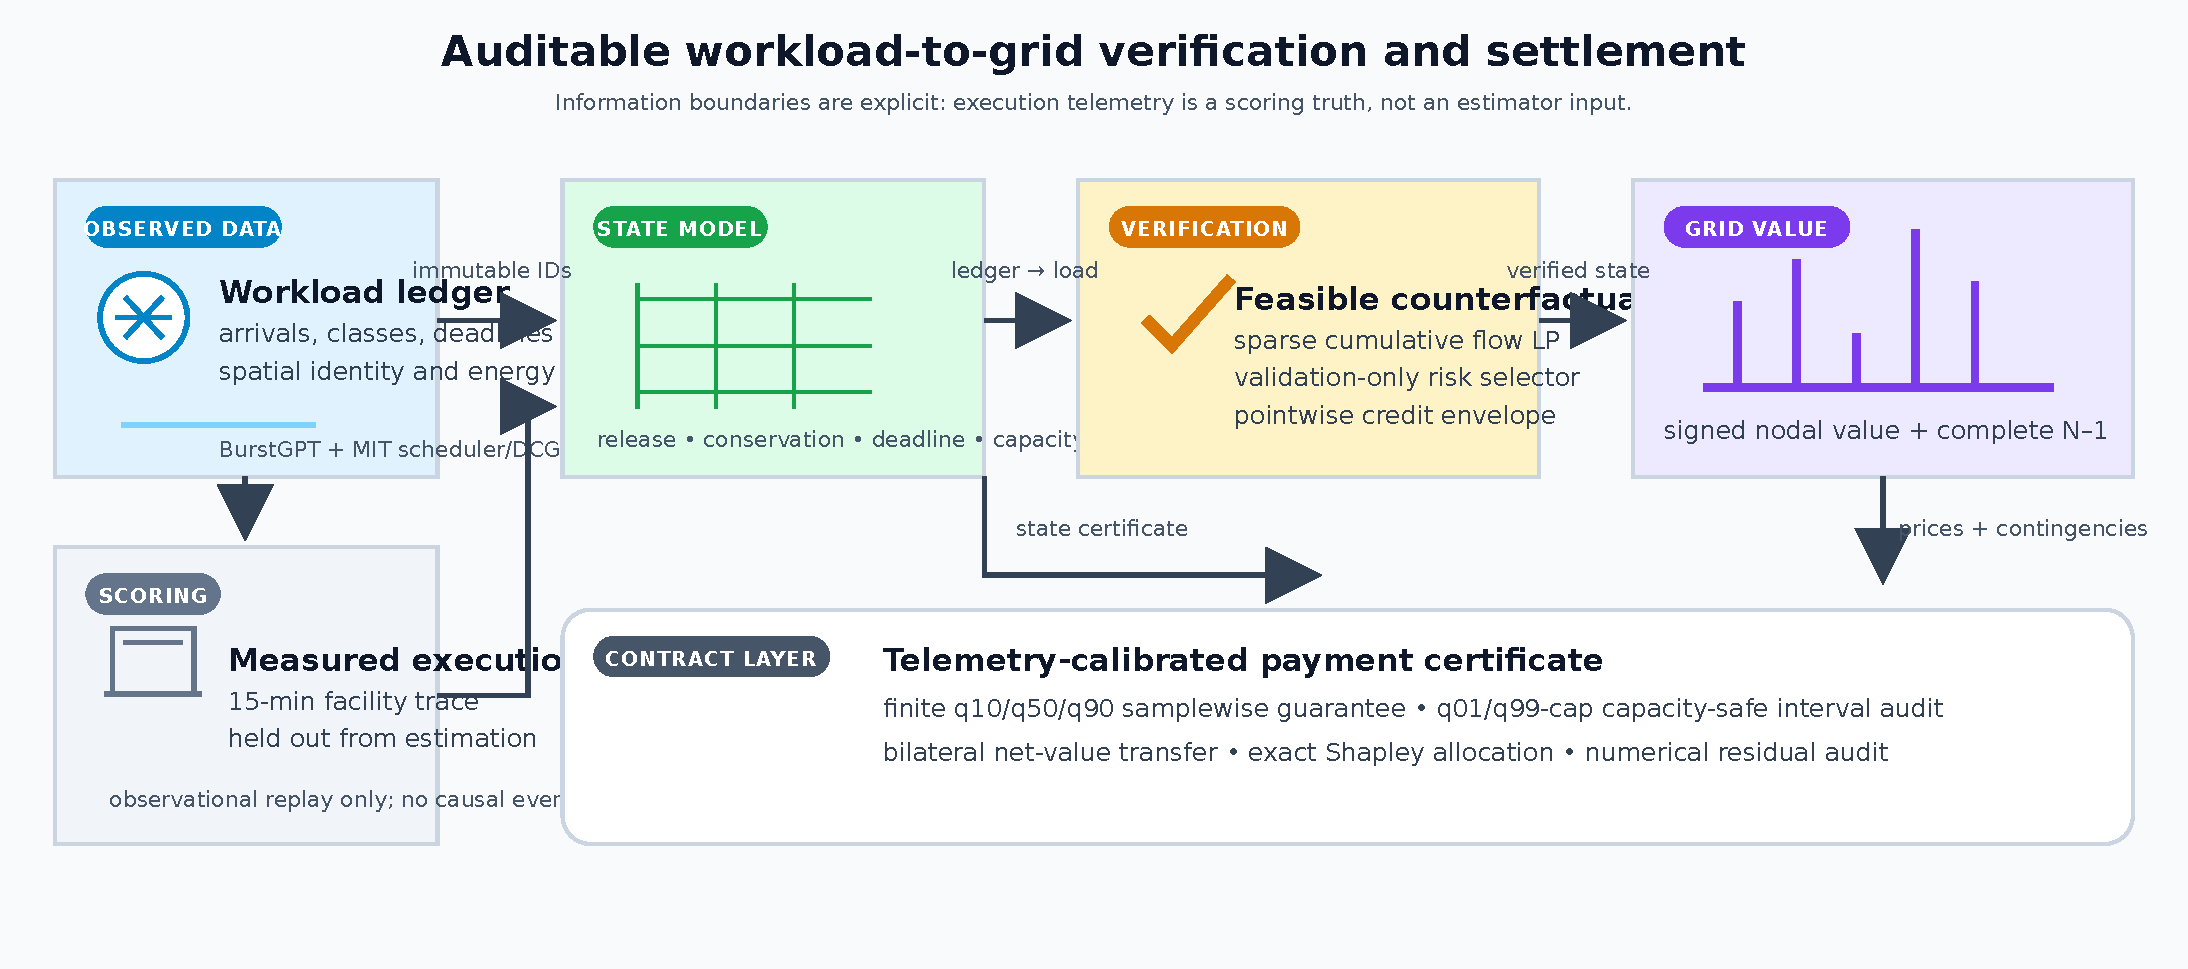
\includegraphics[width=0.90\textwidth]{figures/fig0_framework.pdf}
\caption{Verification-to-settlement framework. Validation labels select the
counterfactual risk contract; locked execution truth is used only for scoring.
The right branch computes aggregate N--1 value and exact participant shares.}
\label{fig:framework}
\end{figure*}

\subsection{Sparse cumulative workload-state verifier}

For statistical estimate $\widetilde p$ and each predeclared penalty $\rho_\ell$,
the first-stage program solves
\begin{equation}
 \min_{x,y,z}\ \mathcal C_{\rm w}(x)+\rho_\ell\sum_{d,t}z_{dt}
 \quad {\rm s.t.}\quad
 z_{dt}\geq\pm(p_{dt}(x)-\widetilde p_{dt}),
 \label{eq:projection}
\end{equation}
subject to (\ref{eq:cumulative})--(\ref{eq:power}). Absolute-value epigraphs
are standard convex constructions \cite{boyd2004convex}; using them to project
a meter baseline onto an auditable workload ledger is specific to this work.
Here $\mathcal C_{\rm w}$ denotes workload operating cost; $C_i$ denotes
generator-segment cost in (\ref{eq:sced}), and $V(p)$ denotes the network
dispatch value. Thus (\ref{eq:projection}) changes the objective, not the
physical feasible set.
Six globally solved schedules $p^{(\ell)}$ share identical arrivals and
constraints. Their validation-only convex combination
$\bar p=\sum_\ell\alpha_\ell p^{(\ell)}$, $\alpha\geq0$,
$\mathbf1^\top\alpha=1$, remains feasible because the common scheduling set is
convex.

The coefficients minimize validation squared error subject to both total and
daily-tail false-credit budgets, where conditional value at risk (CVaR)
measures the latter \cite{rockafellar2000cvar}. Let $\ell^\star$ be the single candidate with
minimum worst contiguous-fold nRMSE and $B_j^{\rm cap}$ its validation false
exposure on day $j$. For reserve $\beta\in(0,1]$,
\begin{align}
 \sum_jF_j(\alpha)&\leq\beta\sum_jB_j^{\rm cap},\label{eq:totalrisk}\\
 {\rm CVaR}_{0.75}(F_j(\alpha))
 &\leq\beta{\rm CVaR}_{0.75}(B_j^{\rm cap}).\label{eq:cvar}
\end{align}
For implementation, the positive part is not differentiated through a sort. For
each event sample $n$ and validation day $j$, the program introduces
$f_n\geq0$, a CVaR threshold $\nu\geq0$, and tail slacks $u_j\geq0$:
 \begin{align}
  f_n&\geq p^\alpha_n-\max\{p^0_n,p^1_n\},\qquad
  F_j=\sum_{n\in j}f_n,\\
  F_j-\nu-u_j&\leq0,\\
  \nu+\frac{1}{0.25J}\sum_j u_j
  &\leq\beta\,\mathrm{CVaR}_{0.75}(B_j^{\rm cap}).
  \label{eq:riskepigraph}
 \end{align}
Together with the simplex equality, box bounds on $\alpha$, and the total
budget in (\ref{eq:totalrisk}), these are linear constraints and the squared
error objective is a convex quadratic program. A HiGHS feasibility solve is
followed by a sparse trust-region solve; the reported KKT and primal residuals
are below $10^{-8}$ in every fitted fold. Four contiguous folds select $\beta$
using validation nRMSE, then risk ratio; held-out noninferiority is reported
as an outcome and is not used as a hidden constraint. A second exact projection targets $\bar p$ while
imposing, for every event sample,
\begin{equation}
 p^{\rm safe}_{dt}\leq p^{(\ell^\star)}_{dt}. \label{eq:envelope}
\end{equation}
\paragraph{Two-sided credit band.}
The upper envelope alone would admit an arbitrarily conservative zero-credit
profile. We therefore impose the matching lower band on the event slots,
\begin{equation}
 p^{(\ell^\star)}_{dt}-\varepsilon
 \leq p^{\rm safe}_{dt}\leq p^{(\ell^\star)}_{dt},
 \qquad (d,t)\in\mathcal D\times\mathcal E,
 \label{eq:twosided}
\end{equation}
where $\varepsilon=1$ MW is fixed before the locked test split. The lower
bound is implemented together with the workload constraints, not as a
post-processing clip. Thus the output remains an attainable schedule while
its credited event trajectory is within a declared band of the selected
single projection. The total constraint (\ref{eq:totalrisk}) controls aggregate
exposure and (\ref{eq:cvar}) controls the worst daily tail; the pair
(\ref{eq:envelope})--(\ref{eq:twosided}) supplies the samplewise credit
certificate. Since $[z-c]_+$ is monotone, the upper inequality bounds false
credit for any unseen actual trajectory, while the lower inequality bounds the
additional under-credit by at most $\varepsilon|\mathcal D||\mathcal E|\dt$
relative to the selected cap. The selected single feasible projection
proves nonemptiness, and the locked results report both margins explicitly.

\paragraph{Decision-time information boundary.}
The ex-post selector can use the complete submitted ledger because it is an
offline settlement protocol. For an event-gate deployment, all arrivals after
the gate are removed before both the causal target construction and optimization,
and terminal completion is required only for work due by the gate. The target is
refit with the same metadata gradient-boosting specification used by the
matched-information baseline, using historical days unchanged and the current
day's masked ledger for every feature row. We additionally solve a committed-ledger safe
mode with $p_{dt}\leq P_d^{\rm fix}$ on the event slots. This mode is an exact
workload LP, uses no future arrivals, and credits only service backed by the
committed ledger; later arrivals become eligible only after commitment. It is
reported separately from the information-boundary diagnostic and the ex-post
benchmark.

The cumulative state reduces the constraint-matrix nonzeros from
$O(|\mathcal S||\mathcal K||\mathcal D||\mathcal T|^2)$ for explicit prefixes
to $O(|\mathcal S||\mathcal K||\mathcal D||\mathcal T|)$. A 512-slot
deadline is handled by (\ref{eq:rollingterminal}) with every observed future
arrival retained; no zero-arrival completion buffer is used in the final
continuous-horizon certificate. The day trajectory is embedded by a
lexicographic pair of linear programs: minimum L1 distance first, followed by
minimum operating cost on that optimal-distance face. Hence no penalty weight
trades physical fit against cost. All linear programs are solved to global
optimality with HiGHS \cite{huangfu2018highs}.
The resulting state-to-credit sequence is summarized in
Fig.~\ref{fig:methoddetail}; the execution replay and interval audit are
reported separately in Experiments 13--15.

\begin{figure*}[t]
\centering
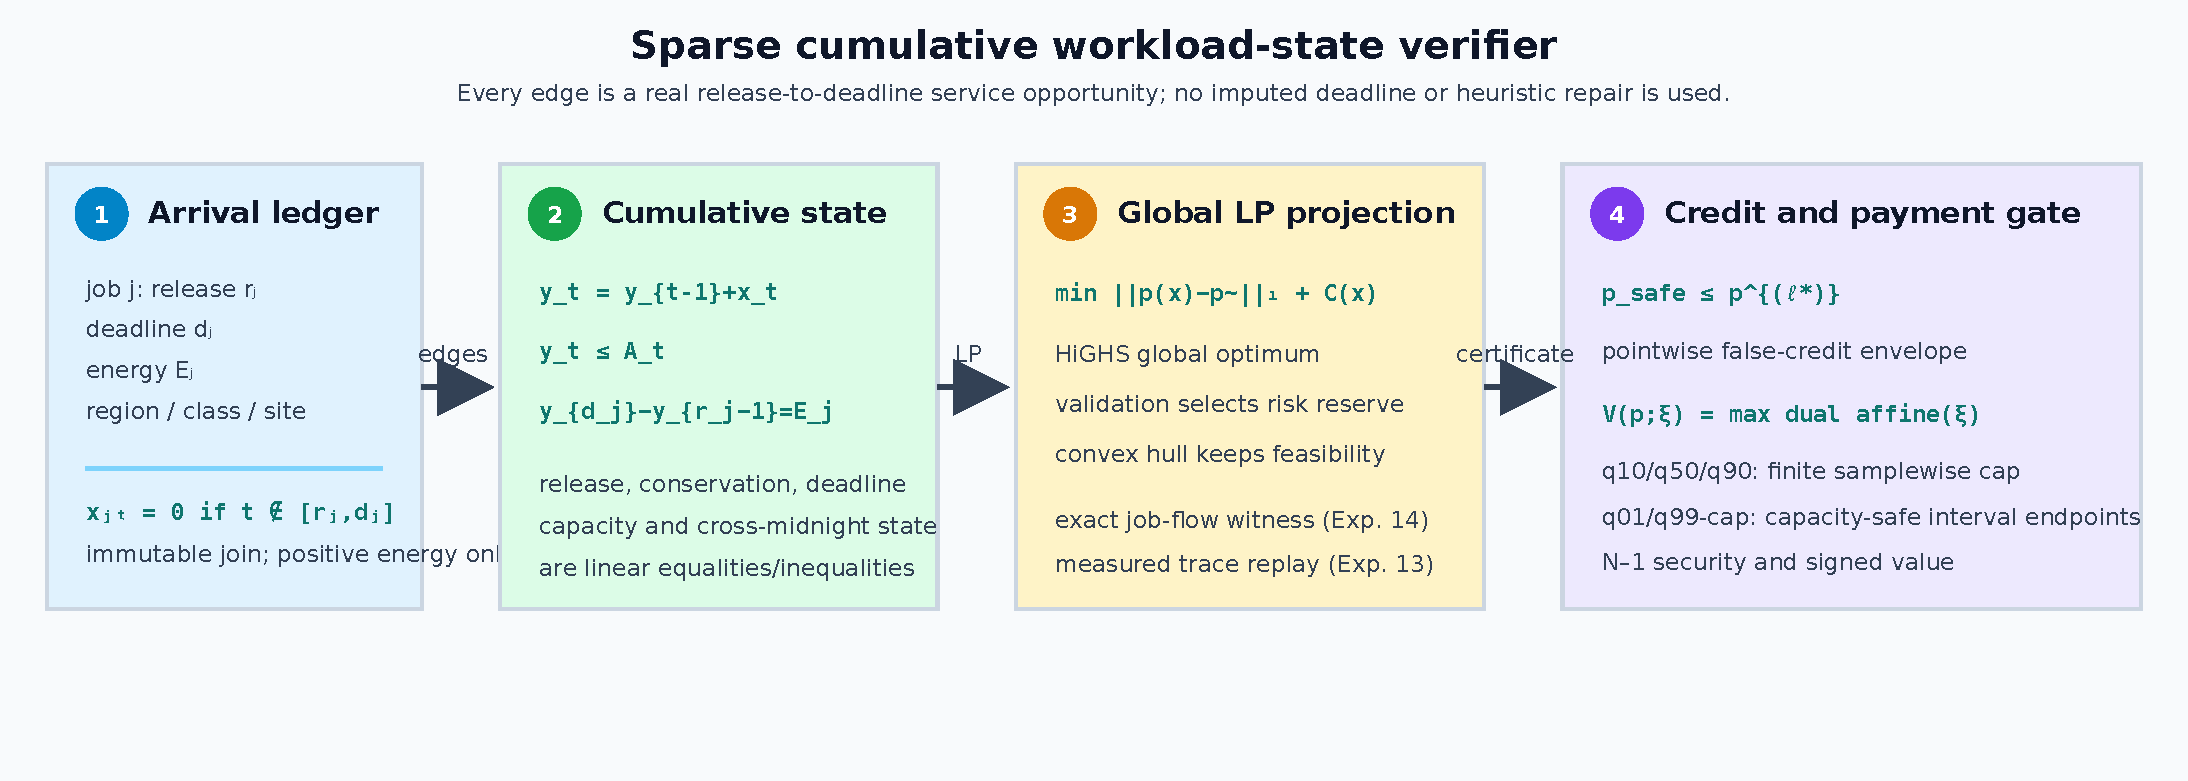
\includegraphics[width=0.90\textwidth]{figures/fig_method_detail.pdf}
\caption{Sparse cumulative workload-state verifier. Real release-to-deadline
edges feed the global feasibility LP; the pointwise credit envelope and the
finite/interval payment gates are applied only after the workload state is
certified.}
\label{fig:methoddetail}
\end{figure*}

\subsection{Signed nodal and N--1 settlement}

Let $\lambda^0\in\partial V(p^0)$ be the nodal demand-value subgradient. Signed
linear settlement is $(\lambda^0)^\top(p^0-p^1)$, while
(\ref{eq:value}) is the realized system-value benchmark and the payoff of an
explicit bilateral avoided-cost contract; it is not relabeled as an independent
system operator (ISO) market
payment. The convex subgradient inequality
\cite{boyd2004convex} yields the global certificate
\begin{equation}
 0\leq(\lambda^0)^\top(p^0-p^1)-\Delta V
 =V(p^1)-V(p^0)-(\lambda^0)^\top(p^1-p^0).
 \label{eq:bregman}
\end{equation}
Thus the linear rule globally upper-bounds exact value in the implemented
polyhedral market model. Equality holds only when both endpoints share a
supporting dual subgradient.

For market-compatible remuneration, let $\mathcal W$ contain the complete
response cycle from the earliest deadline-feasible anticipatory shift through
the latest recovery interval. The space--time rule is
\begin{equation}
 \Pi^{\rm ST}=\dt\sum_{t\in\mathcal W}\sum_d
 \lambda^0_{dt}(p^0_{dt}-p^1_{dt}).
 \label{eq:spacetime}
\end{equation}
This is the nodal virtual-link remuneration structure of
\cite{zhang2020virtuallinks,zhang2022remunerating}, applied here to a verified
counterfactual. Summing site payments reproduces (\ref{eq:spacetime}) exactly.

Space--time energy remuneration is only one component of the contracted DR
product. Let $\mathcal D^{\rm part}$ be the predeclared participating sites,
$\mathcal E$ the event intervals, and $r^{\rm DR}$ the cleared service price.
The signed delivered capacity service and total operator value are
\begin{align}
 Q^{\rm cap}&=\dt\sum_{d\in\mathcal D^{\rm part}}\sum_{t\in\mathcal E}
 (p^\emptyset_{dt}-p^1_{dt}), \label{eq:capacityservice}\\
 G&=r^{\rm DR}Q^{\rm cap}+\Pi^{\rm ST}, \label{eq:operatorvalue}
\end{align}
where $p^\emptyset$ is the minimum-cost no-event schedule under the identical
continuous arrival window. Capacity credits and ex-post participation
constraints follow established DR mechanism design
\cite{satchidanandan2023twostage,chen2021incentive}; the signed
$\Pi^{\rm ST}$ term separately debits spatial transfer and recovery.
Equations (\ref{eq:capacityservice})--(\ref{eq:operatorvalue}) jointly define
the signed service and operator value.

 Let $x^1$ and $x^\emptyset$ denote the workload service schedules inducing
 $p^1$ and $p^\emptyset$, respectively. Define
 $C_{\mathrm{opp}}=\mathcal C_{\rm w}(x^1)-\mathcal C_{\rm w}(x^\emptyset)$ as the participant opportunity
 cost and $S=G-C_{\mathrm{opp}}$ as the transferable transaction surplus. With
 disagreement utilities
equal to zero, the symmetric Nash solution \cite{nash1950bargaining} activates
the contract iff $S\geq0$ and sets
\begin{equation}
 z=\mathbb I\{S\geq0\},\quad
 P^{\rm B}=z\left(C_{\mathrm{opp}}+\frac{S}{2}\right),\quad
 u_{\rm dc}=u_{\rm op}=z\frac{S}{2}.
 \label{eq:nashcontract}
\end{equation}
Thus voluntary nonactivation is the outside option rather than an omitted
outcome. For every activated contract, both utilities are nonnegative and the
single transfer $P^{\rm B}$ is exactly budget balanced. The bilateral transfer
is reported separately from both ISO nodal remuneration and the exact dispatch
value benchmark.
Unlike event-only accounting, $\mathcal W$ debits both pre-event load increases
and delayed rebound; workload conservation gives
$\sum_{d,t\in\mathcal W}(p^0_{dt}-p^1_{dt})\dt=0$ up to solver tolerance.

Security-aware settlement augments (\ref{eq:sced}) with every finite
non-islanding single-line outage. If $L_{\ell k}$ is the LODF from outage $k$
to monitored line $\ell$, then
\begin{equation}
 -\bar f_\ell\leq
 (H_\ell+L_{\ell k}H_k)(C_gg-p)\leq\bar f_\ell,
 \quad \ell\neq k.
 \label{eq:n1}
\end{equation}
Equation (\ref{eq:n1}) is the standard preventive N--1 LODF formulation
\cite{tejada2018lodf}; the experiment enforces all credible rows
simultaneously, rather than screening contingencies. Native public ratings are
retained. Islanding outages are reported and excluded because a connected
single-reference PTDF cannot represent separate islands, consistent with the
scope of DC security models and the N--1 planning criterion
\cite{nerc2020tpl}.

\subsection{Scenario-robust N--1 payment certificate}

The pointwise envelope controls credited energy but does not by itself certify
network payment because spatially different demand vectors can activate
different security constraints. Let $\mathcal P=\operatorname{conv}
\{p^{(1)},\ldots,p^{(L)}\}$ be the convex hull of complete workload-feasible
schedules and let $p^{\rm cap}\in\mathcal P$ be the validation-selected
single feasible projection. Its penalty $\rho_{\ell^\star}$ is selected by
contiguous validation and is reported separately from the payment-target
penalty. The feasible-quantile projection is retained as an external
matched transfer comparator in Section~V. Let $\Xi_3$ contain the 10th, 50th, and 90th percentiles of
held-out per-job measured-to-predicted GPU energy. These predeclared empirical
scenarios define the finite power-conversion contract supported by independent
telemetry \cite{samsi2021supercloud}. For each settlement day, the
\PaymentSafe{} defines
$B_\xi^{\rm cap}=\dt\sum_{t\in\mathcal E}
V_{N-1}(p_t^{\rm native}+M\xi p_t^{\rm cap})$ and solves
\begin{align}
\operatorname{lexmin}_{\alpha,e,\eta,\{g_t^\xi\}}\quad&
 \left(\sum_{d,t\in\mathcal E}e_{dt},-\eta\right)
 \label{eq:paymentcert}\\
\mathrm{s.t.}\quad&
 p^\alpha=\sum_{\ell=1}^{L}\alpha_\ell p^{(\ell)},\nonumber\\
&\alpha\geq0,\quad\mathbf1^\top\alpha=1,\quad 0\leq\eta\leq1,\nonumber\\
&e_{dt}\geq\pm(p^\alpha_{dt}-p^{\rm safe}_{dt}),\nonumber\\
&g_t^\xi\ \text{satisfies (\ref{eq:sced}) and (\ref{eq:n1})},\nonumber\\[-2pt]
&\hspace{2em}\text{with }p_t=p_t^{\rm native}+M\xi p^\alpha_t,\nonumber\\[-2pt]
&\hspace{7.5em}t\in\mathcal E,\quad \xi\in\Xi_3,\nonumber\\
&\dt\sum_{t\in\mathcal E}\sum_iC_i(g_{it}^\xi)\nonumber\\[-2pt]
&\hspace{2em}\leq(1-\eta)B_\xi^{\rm cap},
\quad \xi\in\Xi_3.\nonumber
\end{align}
Generator costs use the same declared piecewise-linear epigraph as market
settlement. Two global linear programs implement the lexicographic objective:
the first obtains the minimum trajectory error, and the second preserves that
optimum within solver tolerance while maximizing the common fractional margin
$\eta$. Existence of the primal dispatches in (\ref{eq:paymentcert}) is
equivalent to the corresponding upper bound on the optimal N--1 value; the
unit weight on $p^{\rm cap}$ proves nonemptiness in every scenario.
Consequently, for any $\xi\in\Xi_3$ and realized event load $p^{1,\xi}$,
daily payment obeys
\begin{multline}
\sum_{t\in\mathcal E}\dt
[V_{N-1}(p_t^{\rm native}+M\xi p^\alpha_t)
-V_{N-1}(p^{1,\xi}_t)]\\
\leq\sum_{t\in\mathcal E}\dt
[V_{N-1}(p_t^{\rm native}+M\xi p^{\rm cap}_t)
-V_{N-1}(p^{1,\xi}_t)].
\label{eq:paymentdominance}
\end{multline}
The common realized-cost term cancels, so the certificate requires no
execution truth and holds samplewise. Both programs contain every finite
non-islanding contingency. The formulation follows the
standard SCED primal and linear-program epigraph foundations
\cite{zimmerman2011matpower,boyd2004convex}.
Here $\mathcal P$ contains the six independently solved first-stage
projections from (\ref{eq:projection}) and the matched feasible-quantile
projection. The \RiskSafe\ is an external target in the absolute-deviation
objective and is not a selectable candidate; the quantile schedule is used
only as an independent transfer comparator, not as the contractual payment
cap.

 The finite cap is complemented by a set-valued payment certificate. The
 contractual cap profile is denoted $p^{\rm cap}=p^{(\ell^\star)}$, where
 $\ell^\star$ is selected by contiguous validation nRMSE; the independent
 payment-target profile $p^{\rm pay}$ is selected separately by validation
 payment error and is used only as the target of the certificate. For a
 realized counterfactual value, define
 $\Delta V_\xi(p)=V_{N-1}(p,\xi)-V_{N-1}(p^{1,\xi})$ and the continuous
 segment $p_\theta=(1-\theta)p^{\rm cap}+\theta p^{\rm cert}$,
 $0\leq\theta\leq1$. The induced interval is
 \begin{equation}
  \mathcal I_\xi=\left[
  \min_{0\leq\theta\leq1}\Delta V_\xi(p_\theta),\;
  \max\{\Delta V_\xi(p^{\rm cap}),\Delta V_\xi(p^{\rm cert})\}\right].
  \label{eq:paymentinterval}
 \end{equation}
 The lower endpoint is obtained by one exact joint N--1 SCED LP with a shared
 segment parameter; the upper endpoint follows from convexity of the optimal
 dispatch value. The selected cap payment is an element of $\mathcal I_\xi$.
 The endpoints use only validation-frozen feasible profiles and the realized
 counterfactual needed for settlement; no oracle baseline selects or certifies
 the interval. Interval width is reported as uncertainty cost, while the
 seven-profile hull remains the finite-scenario payment certificate in
 (\ref{eq:paymentcert}).

\subsection{Participant allocation}

For participants $N$, define $v(S)$ as signed dispatch value when coalition
$S$ moves from baseline to actual demand and nonmembers remain at baseline.
The exact allocation is
\begin{equation}
 \phi_i(v)=\sum_{S\subseteq N\setminus\{i\}}
 \frac{|S|!(|N|-|S|-1)!}{|N|!}
 [v(S\cup\{i\})-v(S)].
 \label{eq:shapley}
\end{equation}
This is the Shapley value \cite{shapley1953value}; the characteristic function
based on signed grid value is the proposed specialization. Grouping
(\ref{eq:shapley}) by coalition size cancels every intermediate value and gives
$\sum_i\phi_i=v(N)$ when $v(\varnothing)=0$. We enumerate all 16 coalitions
for four sites and all 256 coalitions for eight contractual portfolios; no
permutation estimator is used. For larger auditable contracts, exchangeable
slices at the same electrical site are grouped by their member count. The exact
sum retains the binomial multiplicity of every labeled coalition and evaluates
only $\prod_g(m_g+1)$ distinct count states. This symmetry reduction remains
the Shapley value and is evaluated through 20 participants.

\subsection{Analytical guarantees}

\noindent\textit{Proposition 1 (manipulation boundary):} Under a ten-day
arithmetic baseline, differentiable one-sided optimal costs, and an interior
feasible increase in at least one reference-day event service, a strictly
profitable local manipulation exists if and only if
(\ref{eq:threshold}) holds. To prove the statement, differentiate
(\ref{eq:profit}) along any feasible reference-day direction. The marginal
payment is the same $q\pi^{\rm DR}/H$ for every day, whereas the least physical
cost is $\min_j c'_j$. A strict excess selects a positive direction on an
argmin day; if no strict excess exists, every nonnegative local direction has
nonpositive first-order profit. Equality admits indifference but does not
imply strict profit. Experiment 1 computes $c'_j$ from the honest program's
right-hand-side dual and solves the strategic program independently, preventing
the behavioral result from being reused as its own certificate.

\noindent\textit{Proposition 2 (workload and two-sided credit feasibility):}
For fixed arrivals, every convex combination of solutions to
(\ref{eq:cumulative})--(\ref{eq:power}) is feasible, and the envelope output
satisfies the deterministic two-sided band (\ref{eq:twosided}) on every event
cell. Consequently, for every possible unseen execution $c_{dt}$, its
false-credit energy is no larger than that of $p^{(\ell^\star)}$, while its
additional under-credit is bounded by
$\varepsilon|\mathcal D||\mathcal E|\dt$ relative to that reference.
Affine equalities are preserved by the simplex coefficients; each linear
inequality is preserved by convexity. The upper inequality in
(\ref{eq:twosided}) and monotonicity of $[z-c]_+$ give
\[
[p^{\rm safe}_{dt}-c_{dt}]_+
\leq[p^{(\ell^\star)}_{dt}-c_{dt}]_+ .
\]
The lower inequality gives
$[c_{dt}-p^{\rm safe}_{dt}]_+
\leq[c_{dt}-p^{(\ell^\star)}_{dt}]_++\varepsilon$.
Summation over sites and event intervals proves both bounds. The result is a
feasibility-and-band certificate determined by the declared constraints and
$\varepsilon$, not by the distribution of the locked test set.

\noindent\textit{Proposition 3 (security-aware value consistency):} For the
piecewise-linear base-case or N--1 dispatch, exact signed settlement equals the
corresponding optimal-value difference and the nodal linear rule upper-bounds
it by (\ref{eq:bregman}). The feasible-set right-hand side is affine in nodal
demand, so the optimal value is convex and piecewise affine. Applying the
subgradient inequality at $p^0$ gives (\ref{eq:bregman}); applying it again at
$p^1$ yields
\begin{align*}
0\leq \Delta V_{\rm lin}-\Delta V
&\leq (\lambda^1-\lambda^0)^\top(p^1-p^0)\\
&\leq\lVert \lambda^1-\lambda^0\rVert_*
\lVert p^1-p^0\rVert .
\end{align*}
The same proof applies after stacking all rows in (\ref{eq:n1}), because they
remain linear. Gross positive-only settlement has no analogous identity:
truncation changes the response vector before it enters the value function.

\noindent\textit{Proposition 4 (robust daily payment noninferiority):} Every solution
of (\ref{eq:paymentcert}) is workload feasible and its exact N--1 payment is no
larger than the contractual cap payment for every realized event trajectory and
every declared $\xi\in\Xi_3$. Workload feasibility follows from Proposition 2.
For each $\xi$, the embedded dispatch is a feasible witness whose cost
satisfies the corresponding last constraint in (\ref{eq:paymentcert});
optimal N--1 dispatch can only have lower cost. Subtracting the same
scenario-specific realized cost gives (\ref{eq:paymentdominance}).
Conditional on the telemetry-derived finite set $\Xi_3$, the proof is
deterministic and contains no test-outcome assumption.

\noindent\textit{Proposition 5 (continuous worst-case interval certificate):}
For a fixed workload profile $p$, the optimal piecewise-linear N--1 dispatch
value $V_{N-1}(p;\xi)$ is convex in a scalar conversion factor
$\xi\in[\xi_{\rm L},\xi_{\rm U}]$. Therefore
\[
\max_{\xi\in[\xi_{\rm L},\xi_{\rm U}]}V_{N-1}(p;\xi)
=\max\{V_{N-1}(p;\xi_{\rm L}),V_{N-1}(p;\xi_{\rm U})\}.
\]
The value function is the supremum of affine dual objectives in $\xi$, hence
convex; a convex function on a compact interval attains its maximum at an
endpoint. If the two endpoint inequalities
$V_{N-1}(p^\alpha;\xi_e)\leq V_{N-1}(p^{\rm cap};\xi_e)$ hold for
$e\in\{\mathrm L,\mathrm U\}$, then the certified candidate also has no
larger worst-case interval cost than the contractual cap. This interval result is a
worst-case bound; pointwise dominance at every interior $\xi$ is asserted
only for the finite set $\Xi_3$ in Proposition 4. Experiment 15 evaluates
the capacity-safe endpoints with the exact four-segment contractual N--1
model, while Experiment 9 independently replays $\Xi_3$ at 40 segments; the
two resolutions are not conflated.

\noindent\textit{Proposition 6 (workload-segment payment interval):} For a fixed
conversion factor and realized counterfactual, the lower endpoint in
(\ref{eq:paymentinterval}) is the exact minimum payment over the declared
continuous segment because the shared segment parameter and all interval-wise
preventive N--1 dispatch variables are solved in one joint LP. The upper endpoint
is the exact maximum because the optimal dispatch value is convex in the affine
profile and a convex function attains its maximum on a compact segment at a
vertex. Thus (\ref{eq:paymentinterval}) is exact for the contractual segment,
not a grid approximation or a claim that the segment contains every physically
possible schedule. Experiment~15 reports the joint-LP minimum, endpoint maximum,
and resulting width at both held-out conversion endpoints; no oracle baseline
selects the segment.

\noindent\textit{Proposition 7 (provenance-bound workload witness):} Suppose the
canonical tuple in (\ref{eq:ledgerdigest}) is computed from the retained
scheduler--DCGM join after the declared duplicate and positive-energy rules.
If the certificate verifies one-to-one joining, release--execution ordering,
raw-to-join energy conservation, and zero LP residuals, then the job-level
flow witness is a feasible representation of that committed ledger. Under the
collision-resistance assumption of SHA-256, any post-commit modification of a
tuple or its canonical ordering changes the digest except with negligible
probability. The statement binds the computational witness to the committed
records; it does not certify that an uncommitted pre-event submission was
truthful. Experiment 16 checks each premise independently and records the raw
source hashes, so the provenance claim is separate from the scheduling solver's
own feasibility status.

\section{Experimental Design}\label{sec:design}

\subsection{Data, preprocessing, and information boundary}

Table~\ref{tab:data} reports the complete data inventory. BurstGPT contributes
5,188,507 successful requests and observed token service
\cite{wang2024burstgpt}. MIT Supercloud contributes scheduler submissions and
independent Data Center GPU Manager energy. The complete positive-energy
scheduler--DCGM join contains 71,128 jobs, of which 68,664 start within the
common 121-day tensor window used by Experiments 1--13
\cite{samsi2021supercloud}. Submission time creates queue arrivals; measured
execution intervals create scoring truth. A held-out GPU-power regression
uses 28,413 observations and obtains $R^2=0.899$, mean absolute error (MAE)
11.22 W, and root-mean-square error (RMSE) 15.82 W. All 99th-percentile
workload scaling factors are fitted on the first 40 complete days of the
training portion; validation and locked-test days are excluded from that fit.
Per-job measured-to-predicted energy ratios define $\Xi_3$ in
(\ref{eq:paymentcert}); no synthetic row replaces an invalid record.
The 68,664 count is the 121-day workload tensor used by Experiments 1--13.
Experiment 14 does not truncate at that tensor boundary: it extends the
deadline horizon to the last observed scheduler completion and retains all
71,128 positive-energy joined jobs for its independent job-level flow witness.

\begin{table}[t]
\centering
\caption{Complete data and evaluation protocol.}
\label{tab:data}
\footnotesize
\begin{tabular}{@{}p{0.26\columnwidth}p{0.66\columnwidth}@{}}
\toprule
Item & Declared use and count\\
\midrule
BurstGPT & 5,188,507 requests; 2.176 billion tokens; inference arrivals and observed service\\
MIT scheduler & 287,173 raw rows; 104 duplicate rows removed, leaving 287,069 canonical rows; submission time, duration, GPU count, and queue state\\
MIT GPU telemetry & 96,893 rows; 68,664 tensor-window jobs and 71,128 full-horizon positive-energy jobs; measured execution energy\\
Time resolution & 15 min; 121 calendar days; 121 valid complete days\\
Evaluation & 16 validation days followed by 54 untouched test days\\
Networks & RTS-24, IEEE-30, IEEE-39, and IEEE-118 for AC/N--1 panels; IEEE-300 is added in the resolution-convergence panel\\
Provenance & Immutable scheduler/DCGM join digest, raw-to-join energy conservation, and measured regional capacity envelope\\
\bottomrule
\end{tabular}
\end{table}

The public traces do not contain utility bus locations. Consequently, the
four-region coupling is a trace-driven benchmark with fixed, predeclared bus
placements and a declared workload-to-power conversion, not a utility field
trial. Immutable row identifiers determine spatial partitions before any
outcome is computed. Held-out measured-to-predicted job-energy ratios span
0.5845--2.6931 (1st--99th percentiles); the contractual interval uses the
capacity-safe upper factor 1.1499 because the raw 99th-percentile scale would
exceed the precommitted 118-MW nameplate. Experiments 9, 11, and 15 retain the
unclipped factor as a calibration stress value rather than treating the
118-MW scale as a measured geographic fact.
This design permits exact repeated mechanism comparisons but does not identify
a particular operator's geography. Public PGLib and MATPOWER/PYPOWER cases
provide topology, capacities, costs, and ratings
\cite{babaeinejadsarookolaee2021pglib,zimmerman2011matpower}. The RTS-24
benchmark follows the published system data \cite{grigg1999rts}.

\subsection{Baselines, parameters, and inference}

Experiment 2 compares High-5-of-10, ridge regression, gradient boosting, Extra Trees,
online metadata gradient boosting, equally informed post-event metadata
gradient boosting, complete-ledger quantile boosting, pre-event synthetic
control, the exact feasible projection of the complete-ledger quantile,
the \TailRisk, the independently selected single feasible projection,
and the \RiskSafe. The first eight are meter/statistical comparators; the
remaining methods receive the declared ledger as appropriate. The \PaymentSafe
is evaluated separately in Experiments 9 and 15 because its N--1 payment
certificate uses a different objective and a frozen candidate hull.
An information-set
audit verifies feature equality and confirms that no method observes execution
truth.

Real-time inference has zero deferral, elastic inference four slots, and batch
GPU work 512 slots. Per-site flexible capacity is 118 MW plus 6 MW fixed
facility demand; the 118-MW nameplate is committed before the validation/test
split and Experiment~16 only reconciles it with the complete observed
MIT/DCGM batch envelope. Six projection penalties
$\{0.03,0.1,0.3,1,3,10\}$ and four risk reserves
$\{0.60,0.75,0.90,1.00\}$ are selected only on validation data. The settlement
uses 10 generator-cost segments and is scored by an independently solved
40- or 80-segment evaluator. All 5,000 bootstrap replicates use moving
three-day blocks \cite{kunsch1989bootstrap}. Paired tests
enumerate all $2^{18}$ signs of 18 nonoverlapping three-day blocks; Holm
correction controls family-wise error \cite{holm1979multiple}.

The nonlinear model-out check uses the standard polar AC optimal power flow
with active/reactive balance, voltage bounds, generator reactive bounds, and
apparent-power ratings \cite{zimmerman2011matpower}. After solving the intact
state, the preventive panel imposes, for every non-reference generator $i$ and
every credible outage $k$,
\begin{equation}
 P_{Gi}^{(k)}=P_{Gi}^{(0)},\qquad i\notin\mathcal G_{\rm ref},\ k\in\mathcal C.
 \label{eq:acplan}
\end{equation}
The reference generator balances only outage-dependent active losses;
$Q_G^{(k)}$ and bus voltages are contingency recourse. Thus
(\ref{eq:acplan}) tests one shared active plan rather than separately optimized
post-contingency active schedules.

The evaluation follows this chain. Experiments 1--2 test the incentive model and
workload-state verifier; Experiments 3--5 isolate settlement design and network
transfer; Experiments 6--7 test active workload constraints and participant
allocation. Experiment 8 evaluates all RTS-24 line outages, Experiment 9 tests
the telemetry-robust payment certificate and freezes its candidate target and
power scale on validation data, Experiment 10 transfers the
counterfactuals to nonlinear AC models, and Experiment 11 exhausts all declared
spatial assignments and power scales. Experiment 12 embeds each submitted
event trajectory in a continuous real-arrival horizon and evaluates
complete-cycle remuneration and bilateral participation. Experiment 13
replays the measured MIT/DCGM batch trace without intervening in the event,
Experiment 14 solves one exact job-level flow LP for all joined jobs, and
Experiment 15 independently audits the locked payment profile over the held-out
$q_{01}$ to capacity-safe-$q_{99}$ conversion interval; the unclipped $q_{99}$
stress factor is retained in the ledger audit. Experiment~16 audits immutable
ledger provenance and reconciles the regional capacity with the same-source
execution envelope. Experiment 17 fixes the information set at the event gate
and compares a decision-time ledger with the complete-ledger audit. Experiment
18 evaluates AC post-contingency recourse across RTS-24, IEEE-30, IEEE-39, and
IEEE-118 for every outage in a deterministic native-case admissibility set.
Each confirmatory comparison uses the same 54 locked days unless a fixed
network audit rule is stated; the case study is explanatory.

\section{Results}\label{sec:results}

\subsection{Incentive boundary and independent verification}

Experiment 1 solves the entire $8\times7$ DR-price/call-probability grid.
The dual threshold (\ref{eq:threshold}) agrees with the independently solved
strategic program in all 56 cells. At \$150/MWh and $q=0.35$, strategic
reference scheduling inflates the event baseline by 4.09 MWh. Of 52.46 MWh
credited, 18.05 MWh is unsupported by physical reduction, giving a
false-credit ratio of 0.344. The profitable region follows the derived
marginal boundary rather than a fitted classifier; the complete grid and its
phase diagram are retained in the experiment output.

Experiment 2 evaluates all twelve methods on 54 later days. Table~\ref{tab:base}
separates the high-recall \TailRisk\ from the settlement-safe output. The
\TailRisk\ improves mean credit $F_1$ from 0.441558 to 0.484219 over the selected
single projection (Holm-adjusted $p=0.000069$); its nRMSE is 0.330795 versus
0.345209, and the block test does not reject equality ($p=0.130165$). The
\RiskSafe\ combines seven
independently feasible candidates without degenerating to one candidate.
Relative to the equally informed feasible-quantile projection, unsupported
credit falls from 2.917471 to 1.826322 MWh/day, a 37.40\% reduction
(Holm-adjusted $p=0.018494$), while nRMSE changes from 0.321370 to 0.345019
(Holm-adjusted $p=0.546875$). The $F_1$ change is 0.508048 to 0.441220
(Holm-adjusted $p=0.000053$), so the result is a selective reduction in
unsupported credit rather than a claim of uniformly better classification.
Against the selected single projection, RiskSafe changes false credit from
1.849211 to 1.826322 MWh/day (1.24\%, Holm-adjusted $p=0.088379$), nRMSE from
0.345209 to 0.345019 ($p=0.273438$), and $F_1$ from 0.441558 to 0.441220
($p=0.295410$); none of these paired tests is significant. The raw quantile learner exposes 24.156 MWh, showing that the principal gain
is the auditable workload-feasible set and its deterministic credit envelope,
not privileged execution truth. The same-ledger literature panel reports
exact implementations of incentive-compatible spatial DR, price-responsive
non-wire scheduling, proactive workload shifting, and aggregator coordination;
its four 54-day means are retained in the baseline ledger rather than
conflated with the proposed selector.

The new risk fit is a convex quadratic program rather than a nonsmooth
sorted-positive-part optimization: the selected reserve is $\beta=1$ after
four contiguous validation folds, and the final fit has KKT stationarity
$9.4\times10^{-10}$ and zero primal residual. On the locked test days, the
final total false-credit exposure is 394.486 MWh-slot versus 399.430 for the
single-projection cap, and its 75\% daily-tail exposure is 24.235 versus
24.588 MWh-slot; both aggregate certificates are satisfied. The two-sided
certificate in (\ref{eq:twosided}) is checked independently for all 54 locked
days and every event cell. With the predeclared 1-MW band, the mean false-credit
exposure is 1.826322 MWh/day and the mean under-credit is 13.446065 MWh/day,
compared with 13.430785 MWh/day for the selected single cap; every upper
and lower pointwise margin is nonnegative. The RiskSafe therefore occupies a conservative point on an explicit
false-credit/under-credit frontier: relative to feasible quantile it reduces
false credit by 37.40\% but increases under-credit by 1.953 MWh/day and does
not improve $F_1$. The pointwise envelope prevents arbitrary downward
collapse relative to the selected single profile, but it does not make the
accuracy tradeoff disappear. We report this cost directly instead of treating
the certificate as a uniform predictive improvement.

The constraint-set ablation isolates the two risk components. Removing both
the total-exposure and CVaR constraints yields 4.679510 MWh/day of false
credit on the locked days; retaining only the total budget gives 2.522774,
retaining only CVaR gives 3.798364, and retaining both gives 2.523496 MWh/day.
The two budgets therefore have distinct effects: total exposure controls the
aggregate false-credit level, whereas CVaR controls the tail without being a
surrogate for the pointwise envelope. These values come from exact convex
programs with the same candidate set and locked scoring trace; the full
two-sided projection is audited separately above.

\begin{table}[t]
\centering
\caption{Locked 54-day counterfactual results (daily means).}
\label{tab:base}
\footnotesize
\resizebox{\columnwidth}{!}{%
\begin{tabular}{lrrrr}
\toprule
Method & nRMSE & False MWh & Under-credit & $F_1$\\
\midrule
High-5-of-10 & 4.214 & 172.709 & 6.833 & 0.144\\
Ridge & 2.772 & 110.666 & 5.625 & 0.235\\
Gradient boosting & 2.351 & 97.057 & 5.330 & 0.246\\
Extra Trees & 3.336 & 132.971 & 6.947 & 0.177\\
Online metadata & 2.133 & 90.589 & 4.663 & 0.264\\
Post-event metadata & 2.124 & 91.603 & 4.559 & 0.267\\
Post-event quantile & 0.944 & 24.156 & 6.618 & 0.532\\
Synthetic control & 2.552 & 101.835 & 8.427 & 0.206\\
Feasible quantile & \textbf{0.321} & 2.917 & 11.493 & \textbf{0.508}\\
Single feasible & 0.345 & 1.849 & 13.431 & 0.442\\
Tail-risk feasible & 0.331 & 2.523 & 11.980 & 0.484\\
Risk-constrained safe & 0.345 & \textbf{1.826} & 13.446 & 0.441\\
\bottomrule
\end{tabular}%
}
\end{table}

The closest domain baselines are implemented on the same locked ledger rather
than represented by generic machine-learning surrogates. Their daily means are
retained in the complete baseline panel: incentive-compatible spatial DR
(nRMSE 3.063, false credit 114.572 MWh, $F_1=0.137$), price-responsive
non-wire scheduling (0.370, 1.549 MWh, 0.411), proactive workload shifting
(0.345, 1.849 MWh, 0.442), and aggregator coordination (0.517, 0 MWh, 0).
The incentive-compatible and flexibility formulations follow
\cite{chen2021incentive,cao2022flexibility}; the receding-horizon and
aggregator implementations follow \cite{zhang2023receding,zhang2024aggregator}.
The complete day-level rows are retained with the released experiment outputs.

Fig.~\ref{fig:verification} reports the complete day-level distributions,
constraint ablation, validation frontier, and independent intervention
robustness. The 5-by-3 capacity/deadline factorial contains 810 optimal
schedules; maximum capacity- and deadline-binding shares are 0.310 and 0.948.
The measured nonzero effects establish that the associated constraints are not
decorative. Matrix nonzeros scale with log--log slope 1.003 over 96--608
intervals, matching the linear-horizon proposition.

\begin{figure}[t]
\centering
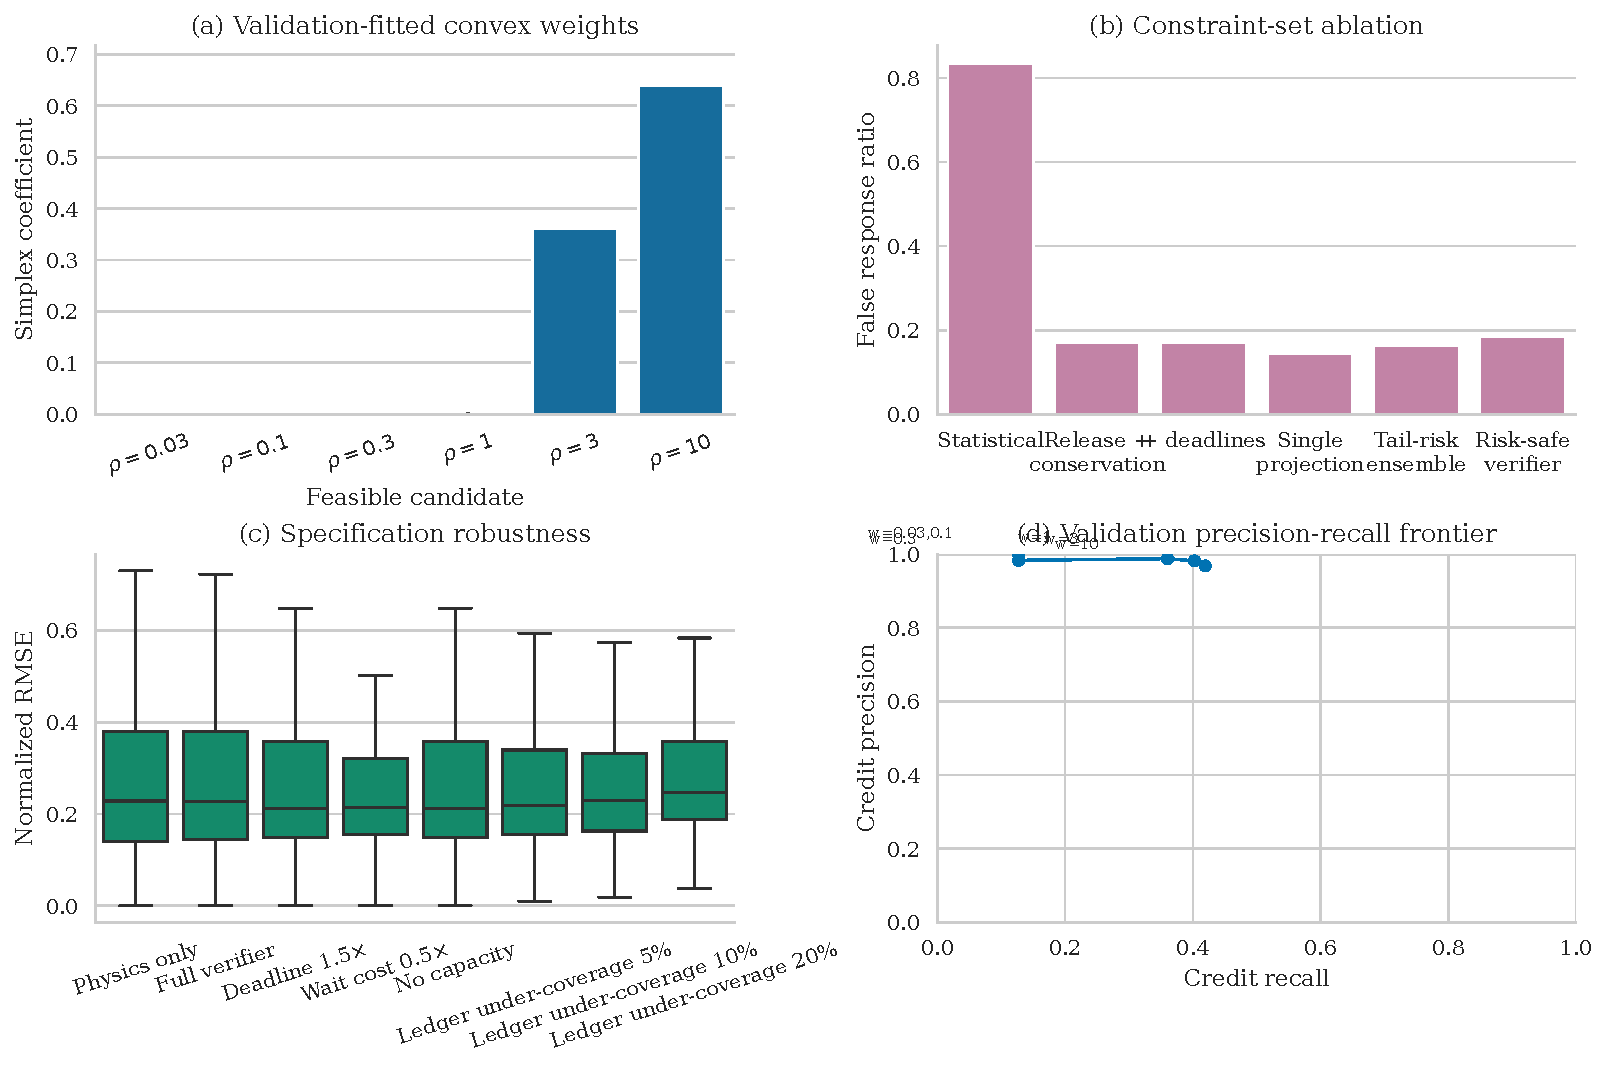
\includegraphics[width=\columnwidth]{../experiments/exp2_baseline_verification/figures/fig4_tuning_and_ablation.pdf}
\caption{Validation-fitted projection weights, constraint-set ablation,
specification robustness, and the precision--recall frontier. Every point is
produced by a globally solved workload program.}
\label{fig:verification}
\end{figure}

\subsection{Nodal value and spatial response}

Experiment 3 crosses thirteen counterfactuals with five settlement mechanisms.
Table~\ref{tab:settlement} first uses the trace-anchored reference to isolate
the mechanism. Exact signed nodal value has mean absolute error \$2.230, versus
\$555.910 for nodal gross response. Under the workload verifier, the errors are
\$454.238 and \$501.324, respectively; the remaining error is dominated by
counterfactual uncertainty rather than value-function linearization.
The paired one-factor decomposition prevents attributing this bundled
improvement to location alone. With the trace reference, signed netting lowers
error by \$551.957/day (Holm-adjusted exact block-sign
$p=8.0\times10^{-6}$), whereas changing uniform signed prices to nodal prices
changes it by only \$0.0032/day ($p=0.4726$), and replacing nodal linear value
by exact value lowers it by \$1.723/day ($p=0.2749$). Under the workload
verifier, the corresponding effects are \$46.958, -\$0.250, and
\$0.128/day; none is a significant universal improvement after the paired
block correction. Thus signed rebound accounting identifies the dominant
trace-layer gain, while end-to-end value differences remain modest and are
tested separately in the congested and N--1 panels below.
All 5,616 interval/counterfactual instances satisfy
(\ref{eq:bregman}); the largest numerical violation is
$2.03\times10^{-11}$ dollars.

\begin{table}[t]
\centering
\caption{Base-case and complete N--1 settlement errors (USD/day).}
\label{tab:settlement}
\footnotesize
\resizebox{\columnwidth}{!}{%
\begin{tabular}{llrrcc}
\toprule
Panel & Settlement & Trace MAE & Workload MAE & Trace median/overpay & Workload median/overpay\\
\midrule
Base case & Uniform gross & 555.923 & 501.511 & -- & --\\
Base case & Nodal gross & 555.910 & 501.324 & -- & --\\
Base case & Uniform signed & 3.956 & 454.116 & -- & --\\
Base case & Nodal signed linear & 3.953 & 454.366 & -- & --\\
Base case & Nodal exact net value & \textbf{2.230} & \textbf{454.238} & -- & --\\
N--1 & Base exact & 165.288 & 192.978 & 85.21/156.62 & 121.75/134.29\\
N--1 & N--1 linear & 2.253 & \textbf{159.514} & 0.59/1.97 & 115.96/38.96\\
N--1 & N--1 exact & \textbf{1.018} & 159.483 & 0.98/0.01 & 116.47/38.37\\
\bottomrule
\end{tabular}%
}
\end{table}

Experiment 4 applies a predeclared rule---the largest gross-minus-net spatial
offset---and selects day 69. The source curtailment, remote rebound, nodal
prices, and line utilization are retained in the experiment output. The case
explains why positive-only local accounting fails: migration creates a
simultaneous negative component that gross payment discards.

\subsection{Cross-network and N--1 security evidence}

Experiment 5 contains 6,480 outcomes over four public networks, three
native-load multipliers, two counterfactual qualities, five mechanisms, and 54
days. Congestion arises endogenously in three of 12 network-load cells. Exact
value improves trace-anchored absolute error in all 12 cells (mean
\$2.126/day; eight Holm-adjusted block tests below 0.05). For the workload
verifier, the exact rule reduces the cell-averaged absolute error from
\$765.776 to \$765.629/day (a \$0.147/day paired reduction); none of the 12
Holm-adjusted tests is significant. This separation supports Proposition 3
without converting a trace diagnostic into an end-to-end dominance claim.

The near-affine RTS-24, 0.98-load cell is recomputed on all 54 days at
10/40, 20/80, 40/160, and 80/320 settlement/evaluation segments. The four
signed-linear-minus-exact differences are $0.010632$, $0.021578$, $0.025515$,
and $0.030576$ USD/day; each remains below $0.04$ in magnitude. The stable,
small effect across resolutions confirms that the observed local-affinity
diagnostic is not a discretization artifact.

Experiment 6 crosses capacity multipliers
$0.55,0.70,0.85,1.00,1.20$ and deadline multipliers
$0.25,0.50,1.00$ over 54 days (810 globally solved schedules). Capacity- and
deadline-binding shares reach 0.0334 and 0.9118, respectively, while the
capacity-level mean false-credit exposures are 2.700, 2.407, 2.303, 2.297,
and 2.407 MWh. Deadline binding remains 0.8738--0.9118 across the three
deadline multipliers. Every schedule satisfies the declared workload
constraints.

Experiment 7 enumerates all 16 coalitions for four participants and all 256 for
eight. Trace-reference Shapley error is zero with maximum budget residual
$2.3\times10^{-13}$ dollars; workload-verifier mean participant error is
$92.519$ dollars while its maximum budget residual is
$1.14\times10^{-13}$. The exchangeable scaling panel reaches 20 participants
(1,296 states; maximum residual $2.27\times10^{-13}$), confirming exact budget
balance rather than permutation sampling.

Experiment 8 enforces (\ref{eq:n1}) for all 37 non-islanding outages of RTS-24
(the single islanding line is reported separately). Over 54 locked days and
2,592 interval-mechanism outcomes, native ratings, 0.90 load, 6\% penetration,
and four fixed sites are held constant; a 10-segment certificate is scored by
an independent 40-segment N--1 dispatch. Trace-anchored mean errors for
base-case exact, N--1 linear, and N--1 exact are \$165.288, \$2.253, and
\$1.018 per day. Exact N--1 improves on base-case exact by \$164.270/day
(Holm-adjusted $p=3.1\times10^{-5}$), whereas its \$1.235/day advantage over
N--1 linear is not significant ($p=0.3518$). Workload-verifier errors are
\$192.978, \$159.514, and \$159.483 (base-to-exact $p=0.3518$;
linear-to-exact $p=0.9309$), showing that the large trace gain does not
translate into a significant end-to-end gain. Maximum post-contingency
utilization is 1.000 p.u.; signed overpayment is retained in Table~\ref{tab:settlement}.

Experiment 9 tests (\ref{eq:paymentdominance}). All 54 daily lexicographic
program pairs attain global optimality; the seven-profile candidate hull is
anchored to the validation-selected single projection $p^{\rm cap}$, while the
payment-target selection is frozen independently. The held-out factors 0.734,
0.996, and 1.278 form $\Xi_3$; all 162 certificates have zero positive cap
violation and mean cost margins \$17.506, \$23.542, and \$30.346/day. The
384-cell validation-only N--1 panel selects the feasible-quantile profile as
$p^{\rm pay}$ (MAE \$53.471), with no locked-test payment or peak outcome used
in that choice. Independent 40-segment replay gives mean absolute payment
errors averaged over $\Xi_3$ of \$194.282/day for \PaymentSafe, \$179.261 for
the selected single projection, \$190.284 for feasible quantile, and \$179.272
for \RiskSafe. These accuracy scores do not replace the deterministic cap.
The maximum post-contingency loading remains 1.000 p.u. Experiment 15
separately audits the capacity-safe closed conversion interval and is
interpreted through Proposition 5. Its exact four-segment continuous-profile
certificate has mean payment-interval width \$13.947662/day at $q_{01}$ and
\$27.210301/day at the capacity-safe $q_{99}$ endpoint (maximum widths
\$92.035916 and \$182.027759/day). The raw held-out $q_{99}=2.6931$ is retained
as an unclipped calibration value but exceeds the precommitted 118-MW nameplate;
the contractual upper endpoint is therefore the ledger-audited safe factor
1.149889. This interval is an explicit uncertainty cost, not a lower-error
claim. The cap is a contractual upper bound under the declared market model;
it is not evidence that the payment-certified profile has lower independent
prediction error than every comparator.

Experiment 10 replaces the linear network with nonlinear AC OPF
\cite{zimmerman2011matpower}. Across RTS-24, IEEE-30, IEEE-39, and IEEE-118,
all 864 base outcomes converge with zero voltage violation and a maximum
apparent-line loading of 1.00000003 p.u.; the numerical excess above one is
$2.1\times10^{-8}$, below the declared $10^{-6}$ AC feasibility tolerance. The
payment guarantee remains scoped to (\ref{eq:paymentcert}). The corrective
panel adds 5,400 OPFs over IEEE-9/14 non-islanding outages and reaches a maximum
loading of 0.8816 p.u. with zero voltage violation. A shared active plan is
then fixed across all six IEEE-9 outages as in (\ref{eq:acplan}); its 3,888
cells converge with zero non-reference active-plan deviation and maximum
loadings 0.878/0.903/0.929 p.u. at 3\%, 6\%, and 9\% penetration. The
corresponding maximum reference-generator loss recourse is 5.455/5.727/6.014
MW.

Experiment 11 removes fixed trace placement and power scale by crossing all
$4!=24$ region-to-bus mappings, 3\%, 6\%, and 9\% peak penetrations, four
counterfactuals, and all 54 days, yielding 15,552 outcomes. The \RiskSafe\
has mean absolute payment errors of \$100.220140/\$201.509173/\$296.950629 per
day at 3\%/6\%/9\% penetration. The matched feasible-quantile projection is
lower-error at \$84.335866/\$169.715274/\$249.216682, whereas \RiskSafe\ is
lower than the independently selected single feasible projection
(\$100.270490/\$201.609873/\$297.101679) in all 72 mapping--scale cells, with
mean advantages of \$0.050350/\$0.100700/\$0.151050 per day. Thus this panel
supports spatial and scale transfer of the risk-bounded profile; it does not
relabel the external quantile comparator as an error-dominated method. The
public IEEE-118 native load is fixed at the predeclared 0.90
multiplier used by the N--1 stress panel, while native branch ratings remain
unchanged. Maximum loading and locational marginal price spread are 1.000 p.u.
and \$4.06/MWh.
The corresponding panels separate the conversion-scenario cap, shared-active-
plan AC envelope, and spatial-scale transfer from the base-case accuracy
results, so these claims are not conflated with the trace-anchored mechanism
isolation result. Experiment 16 adds a direct calibration sensitivity: held-out
measured-to-predicted energy ratios are 0.5845, 0.7342, 0.9957, 1.2780, and
2.6931 at the 1st, 10th, 50th, 90th, and 99th percentiles. Applied to the
flexible MIT batch envelope, the direct q90 and q99 scales exceed the 118-MW
commitment (131.149 and 276.361 MW before clipping); the released sensitivity
file reports the capacity-safe clipped factor (1.149889 at both endpoints)
separately from the validation-frozen
3\%--9\% network panel. This
is a calibration bound, not a claim that public traces identify a field
geography. The complete assignment--penetration panel is retained in the
experiment output.

Experiment 12 removes the daily reset: each event is embedded in 1,216 slots
(608 pre-event, 96 event, 512 recovery), with only the eight event intervals
projected. Across 216 method--day outcomes, maximum event L1 and cycle-energy
residuals are $6.0\times10^{-6}$ MW and $3.0\times10^{-6}$ MWh. Complete-cycle
MAE is \$0.084761/event for \PaymentSafe, \$0.053170 for feasible quantile,
\$0.241926 for \RiskSafe, and \$0.084761 for single projection; event-only MAE
is \$8.091153, \$11.655725, \$11.186565, and \$10.763272. Mean verified
capacity is 13.902285 MWh at \$150/MWh; all 54 Nash contracts activate (mean
surplus \$2,034.810894; minimum utility \$1.842918), with site residual below
$1.42\times10^{-14}$. Table~\ref{tab:rolling} reports the cycle certificate.

\begin{table}[t]
\centering
\caption{Continuous rolling-horizon market validation over 54 locked days.}
\label{tab:rolling}
\footnotesize
\resizebox{\columnwidth}{!}{%
\begin{tabular}{lrrrr}
\toprule
Metric & \PaymentSafe & Quantile & \RiskSafe & Single \\
\midrule
Complete-cycle MAE (\$/event) & 0.084761 & 0.053170 & 0.241926 & 0.084761 \\
Event-only MAE (\$/event) & 8.091153 & 11.655725 & 11.186565 & 10.763272 \\
Max window residual (MW) & \multicolumn{4}{c}{$6.0\times10^{-6}$} \\
Max cycle-energy residual (MWh) & \multicolumn{4}{c}{$3.0\times10^{-6}$} \\
Verified capacity (MWh) & 13.902 & 13.902 & 13.902 & 13.902 \\
Positive contracts & \multicolumn{4}{c}{54/54} \\
\bottomrule
\end{tabular}%
}
\end{table}

\subsection{Independent trace and deployment-boundary audits}

The independent audit separates measured execution from the semi-synthetic
intervention. Replaying immutable MIT scheduler/DCGM intervals over 54 days
gives slot MAE 3.744 versus 5.764 MW for the batch-only trace and 100\% slot
coverage; the corresponding mean absolute energy discrepancies are 359.459 and
553.380 MWh. This is observational fidelity, not a causal event. A sparse flow LP
retains all 71,128 positive-energy jobs (1,974,690 service variables),
reconstructs 2.657346 MWh, and has residuals below $10^{-17}$ MWh. The raw
execution peak is 0.006685 MW; the train-fitted scaled benchmark envelope peaks
at 102.619 MW (0.870 of the precommitted 118-MW nameplate). The q90 and q99
conversion sensitivities exceed that nameplate before capacity-safe clipping.
These results establish ledger fidelity and make the scaling interpretation
explicit; they do not turn the public trace into a utility measurement or
establish semantic-field authenticity.

\begin{table}[t]
\centering
\caption{Independent replay, interval-payment, and ledger-provenance certificates.}
\label{tab:replay-flow}
\footnotesize
\resizebox{\columnwidth}{!}{%
\begin{tabular}{llll}
\toprule
Evidence & Quantity & Baseline / value & Verified result \\
\midrule
Trace replay & Mean slot MAE (MW) & Batch-only 5.764 & Trace-constrained 3.744 \\
Trace replay & Mean energy discrepancy (MWh) & Batch-only 553.380 & Trace-constrained 359.459 \\
Trace replay & Slot coverage & -- & 100\% over 54 days \\
Flow witness & Jobs / service variables & -- & 71,128 / 1,974,690 \\
Flow witness & Energy / maximum residual & -- & 2.657346 MWh / $9.4\times10^{-18}$ MWh \\
Capacity & Raw execution / scaled benchmark peak & -- & 0.006685 / 102.619 MW (0.870 of nameplate) \\
Interval certificate & Endpoint margins $q_{01}/q_{99\text{-cap}}$ & -- & \$13.948 / \$27.210 per day \\
Interval certificate & Maximum cap violation & -- & $2.9\times10^{-9}$ USD \\
\bottomrule
\end{tabular}%
}
\end{table}

The held-out conversion-interval audit evaluates $q_{01}=0.5845$ and the
capacity-safe upper endpoint $q_{99\text{-cap}}=1.149889$ with the exact
four-segment certificate model; the raw $q_{99}=2.6931$ is retained as a
calibration stress value and is clipped by the precommitted 118-MW nameplate.
The continuous-segment widths are $\$13.947662$ and $\$27.210301$ per day,
with maximum widths $\$92.035916$ and $\$182.027759$. Proposition 5 therefore
certifies the worst-case cost over the declared capacity-safe closed interval.
The decision-time audit removes all post-gate
arrivals before both optimization and target construction: the truncated-ledger
diagnostic has nRMSE 0.451393, false credit 1.257628 MWh/day, and credit
recall 0.032868, whereas the complete-ledger
RiskSafe has nRMSE 0.345019 and recall 0.353429. The committed-ledger
pointwise-safe mode has zero false-credit exposure and zero event-credit recall
by design because it does not credit uncommitted future work. Finally, 1,698 declared AC
corrective recourse rows are solved across four public networks and three
validation-scaled penetrations. These are model and information-boundary
audits, not a preventive AC security-constrained OPF certificate or a
field-event result.

\section{Conclusion}\label{sec:conclusion}

This paper develops a provenance-bound workload-state verifier and a
security-aware nodal settlement for spatially coupled AI data centers. The
cumulative state enforces release, deadline, conservation, migration, and
capacity constraints; the convex risk program uses an explicit linear
false-credit/CVaR epigraph; the two-sided credit band limits unsupported
credited response and bounds additional under-credit; and signed N--1 value
accounts for rebound and congestion. Across 54 locked days, false-credit
exposure is 1.826322 MWh/day for RiskSafe, compared with 1.849211 for the
selected single cap and 2.917471 for feasible quantile; its nRMSE is 0.345019
versus 0.345209 and 0.321370, respectively. The same comparison increases
under-credit by 1.953 MWh/day relative to feasible quantile and does not improve
$F_1$, so the empirical result is a risk tradeoff rather than uniform predictive
dominance. The trace-anchored mechanism-isolation panel reduces N--1
exact-settlement error from \$165.288 to \$1.018/day, whereas the end-to-end
workload-verifier errors are \$192.978, \$159.514, and \$159.483/day for the
base-case exact, N--1 linear, and N--1 exact variants; the latter difference is
not significant under the block test. The job-level witness preserves 71,128
measured jobs with machine-precision residuals, and the provenance certificate
binds the witness to the immutable scheduler/DCGM join and reconciles the
precommitted 118-MW nameplate with a clearly separated raw execution and scaled
benchmark envelope. The
committed-ledger event-gate mode has zero false-credit exposure but credits no
uncommitted future work; the interval payment audit reports the resulting
conversion uncertainty instead of hiding it. Held-out calibration sensitivity
and the cross-network AC audit evaluate the declared capacity and topology
boundaries. The public traces provide reproducible workload and network
evidence rather than a utility field intervention. Deployment therefore
requires a signed operator ledger, co-located facility telemetry, topology
access, and a capacity-safe workload-to-power conversion; these requirements
define the next intertemporal AC and utility-event validation stage.

\bibliographystyle{ieeetr}
\begingroup
\fontsize{6.5pt}{7.1pt}\selectfont
\bibliography{references}
\endgroup

\end{document}
